% Chapter Template

\chapter{Results and Discussion} % Main chapter title

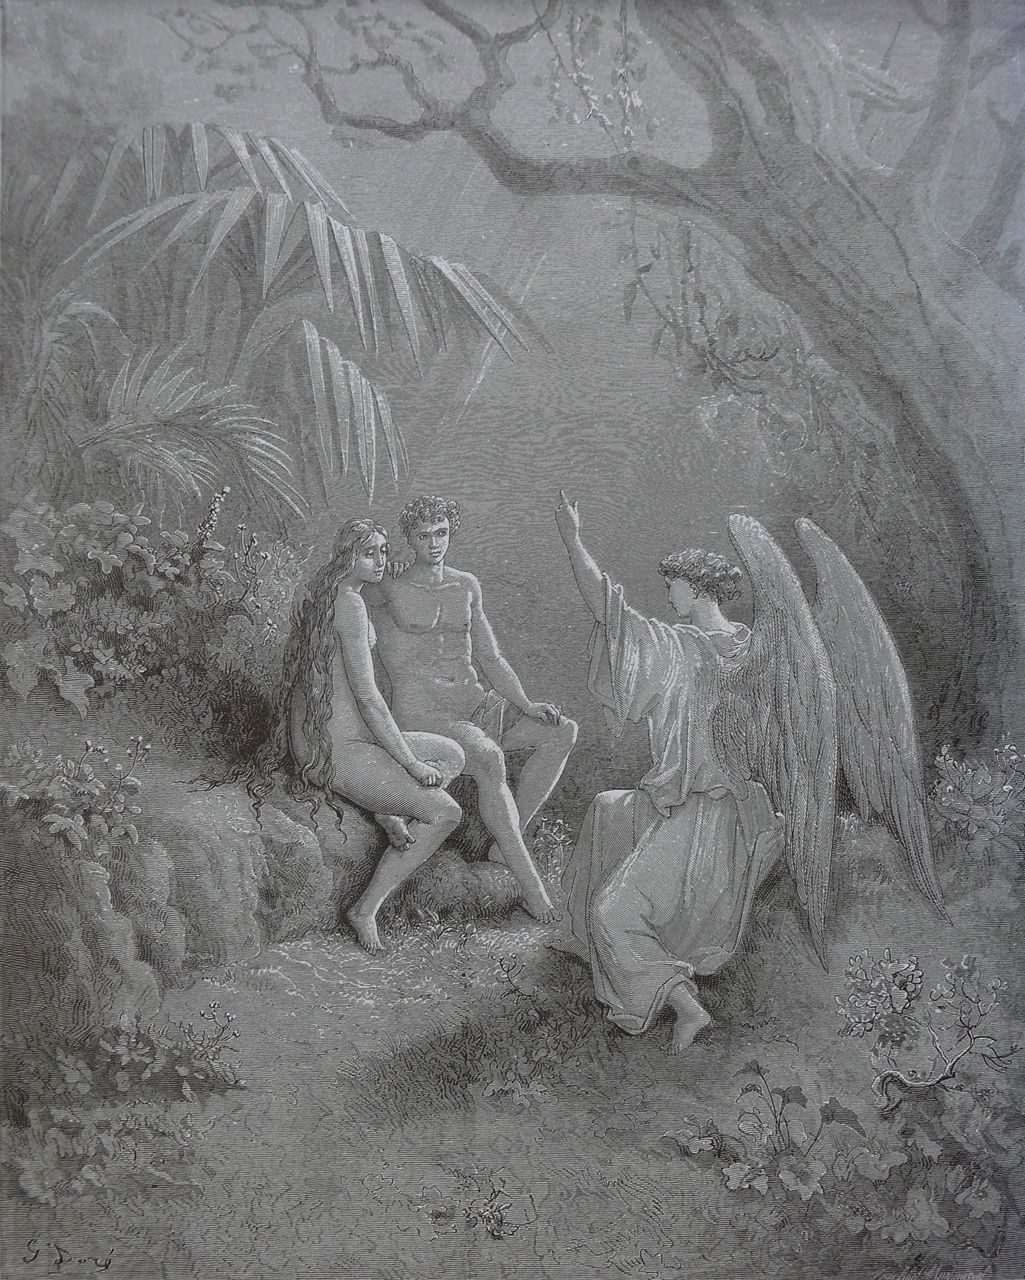
\includegraphics[width=\linewidth,trim={0 7cm 0 12cm},clip]{Paradise_Lost_22}

\label{Chapter 7} % Change X to a consecutive number; for referencing this chapter elsewhere, use \ref{ChapterX}

\section{Overview}

In the following chapter what was achieved over the project will be discussed. This will begin with the challenges encountered during and final state of the matrix mode and secure compartment sections. This will then continue on to discussing the research questions and will end with a discussion about the future works of the project regarding matrix mode and the secure compartments.

%----------------------------------------------------------------------------------------
%	SECTION 1
%----------------------------------------------------------------------------------------

\section{Matrix Mode Operation}

\label{Ch7 Sec1}

When initially starting the project, matrix mode was in a unusable state. The serial interface with the device was locked after input, only allowing a single character to be read. In addition to the locking, there were several visual issues that inhibited the function of matrix mode. While these issues were corrected over the course of the project, they did come with their own challenges along the way. 

%-----------------------------------
%	SUBSECTION 1
%-----------------------------------
\subsection{New Developer Issue}

\label{Ch7 Sec1 Sub1}

The biggest issue encountered when attempting to correct any of the parts of matrix mode was the lack of comments. This project has multiple developers in it and while some sections are well documented, there are some sections that are not obvious to new developers.\\
In addition to the lack of foundation available, the range of development tools in use in this project requires an advanced knowledge of programming and hardware design. Throughout this project the design language VHDL was the main language used, but despite this a detailed knowledge was required of Verilog, GS4510 assembly, Vivado tool command language (tcl) and Make. As I had no knowledge of the latter languages this made some sections of the project difficult to design.\\
Despite these challenges changes to the tcl, Make and Assembly files were able to be done and an understanding of the Verilog files was developed.

%-----------------------------------
%	SUBSECTION 2
%-----------------------------------
\subsection{Serial Locking Issues}

\label{Ch7 Sec1 Sub2}

During the correction of the serial locking issue, correcting the offending code proved to be very challenging. As the MEGA65 did not have all the excessive resources of modern devices, after identifying the issue, it was difficult to implement a solution to the problem that was efficient. This lead to brainstorming of possible corrections and their security implications. In the end, the solution that was favoured was the edit code that was already present, adding the minimal amount of my own code. This issue was entirely overcome after implementing the first change to the MEGA65. Upon suggesting my change to Dr. Gardner-Stephen I was informed that any change made should be added to the project. This was as the optimisation of the device had not yet occurred, so any changes I make will inevitably be improved.  

%-----------------------------------
%	SUBSECTION 3
%-----------------------------------
\subsection{Letterboxing}

\label{Ch7 Sec1 Sub3}

During the correction of the visual issues in matrix mode through a letterbox signal, a lack of project knowledge proved to be very tough to overcome. This lack of knowledge resulted in several attempts to correct the issue through offsets and other, ultimately useless, tricks to move the terminal memory around. If a greater knowledge of the other sub-systems in the MEGA65 was possessed then the corrections to the device would have proceeded more rapidly.

%-----------------------------------
%	SUBSECTION 4
%-----------------------------------
\subsection{Visual Bug Chasing}

\label{Ch7 Sec1 Sub4}

During corrections to the visual bugs, the biggest challenges faced were the exposing of signals and understanding of what was happening. While running the hardware, exposure of the signals was difficult due to the limited amount of LEDs on the board. This made identification of some of the bugs slow. To combat this, GHDL, the VHDL simulator was used. This exposed the signals more readily as there were report statement littered through the project, this would make signal tracking trivial. GHDL, unfortunately, did not provide a graphical display of what was occurring on the hardware, making discrimination of expected behaviour from unexpected behaviour difficult.

%----------------------------------------------------------------------------------------
%	SECTION 2
%----------------------------------------------------------------------------------------

\section{Secure Compartment Implementation}

\label{Ch7 Sec2}

\subsection{SD card Fixing}

\label{Ch7 Sec2 Sub1}

Fixing the SD card functions, as described in section \ref{Ch6 Sec2 Sub2}, was where the first major issue in the project was encountered. This was due to the multiple branches of knowledge required to even verify id the SD card was working or not. Firstly, a knowledge of the VHDL files was required, in addition to this, knowledge of where the SD card was saving and reading from was required. This allowed me to understand how reading and writing was occurring. But to check that they were occurring correctly, I needed to understand and use assembly to query the CPU through the matrix mode commands. This allowed me to manually write, read and reset the SD card.

\subsection{Hypervisor Trap}

\label{Ch7 Sec2 Sub2}

During the creation of the hypervisor trap for secure mode a communication error occurred between Dr. Gardner-Stephen and I. I believed that the hypervisor traps were all done in hardware, as there were hardware implementations for some hypervisor traps in the CPU. This was not the case, the majority of hypervisor traps were to be executed in software. This miscommunication resulted in a time loss on the project.

\subsection{Secure mode Entry/Exit}

\label{Ch7 Sec2 Sub3}

During implementation of the secure mode entry and exit the biggest challenge of the project was encountered. The sequencing for events and interactions between the various sub-systems required very careful consideration. As discussed in section \ref{Ch6 Sec4 Sub1}, in order to eliminate the possibilities of exploitation control needed to be taken away from the user to make certain processes atomic.

%----------------------------------------------------------------------------------------
%	SECTION 3
%----------------------------------------------------------------------------------------

\section{Research Question Satisfaction}

\label{Ch7 Sec3}

\textit{What are the missing or non-functional sub-systems that the MEGA65 requires to be implemented?}\\
Over the course of the project, several missing and/or non-functional sub-systems were found within the MEGA65 smart phone. 
Of those sub-systems, the ones that were fixed are detailed in chapters \ref{Chapter 4}, \ref{Chapter 5} and \ref{Chapter 6} of this document. 
Despite the fixes applied, there are still many sub-systems of the phone that require additional attention in order for them to function as intended.\\

One of the functions of the phone is being able to create and load save states that are images of the phone at a particular point in time. These save states are mostly functional, but there are still some strange cases, in which, their functionality is not entirely as expected or missing. It was noted, but not explored, that creating a save state in the most recent version of the phone causes the partition table to be invalidated. This is suspected to be the result of some change to the save state code causing the slot pointer to point to the partition table instead of the desired slot.\\

The save state error also has a cascading effect into the implementation of secure mode, as discussed in chapter \ref{Chapter 6}. 
As described in section \ref{Ch6 Sec3 Sub2}, the secure mode implementation plans to use this save state process as a part of it, this error will therefore cause the secure state to corrupt the partition table.\\

In addition to the partition corrupting, the secure mode is also non-functional for a number of other reasons. 
The string comparison seen in figure \ref{fig:monitoracceptreject}, only compares the input to the upper case version of accept or reject. 
While this could be intentional to ensure that the user truly desires the result, by entering reject in lower case an instruction is invoked. 
This is due to the lower case 'r' character being an instructional prefix. 
Another issue with secure mode was when successfully rejecting secure compartments. When the SD card has been removed from the device, there is currently no protection to stop the phone from loading despite this.
This causes the secure mode to load from nothing and produces unpredictable results.\\

Although functionality to matrix mode has mostly been restored, it is not working entirely as intended. 
From within matrix mode it is possible to halt and single step the CPU, if the CPU is halted, then a request to leave matrix mode is sent and stepped through, the user is left in user mode with a frozen CPU and no way to return to matrix mode.
When exiting from matrix mode with the secondary exit keycode, superkey + ~, the ~ key is printed in user mode. 
This is believed to be due to double scanning of the non-special input keys.\\

When experimenting with the SD card compatibility, it was noted that the SDXC card was not recognised as an SD card at all. Investigation into the SD card hardware showed that there was no case for this type of card. 
In addition to this, in the latest version of the phone, the SD card detection no longer rescans for the SD card if one is not initially detected.\\
\\
\textit{How can these sub-systems be implemented?}\\
\begin{itemize}
\item{Load and Save Sate}\\
  The save state partition table corruption issue should be solved by reviewing the location at which the save state is attempting to be saved to. 
  This location should be confirmed as save state slot. 
  Additionally, the size of the data being saved should be compared to the size of the save state slot to ensure that other data is not being overwritten.
\item{ACCEPT/REJECT Strings}\\
  To ensure the secure compartment sub-system is functional and in accordance with the user's expectations, the lower case versions of accept and reject should also have the same functionality as the upper case versions. 
  Conversely to this, if the accept and reject cases are restricted to upper case only, inputting a lower case version should send a warning to the user and, in the reject case, not throw a syntax error.
\item{CPU Locking}\\
  To prevent CPU locking and restore some functionality to matrix mode, exiting matrix mode should be tied into unfreezing the CPU.
\item{SD card Protection}\\
  To protect the SD card against loading junk data from the SD card slot when the SD card is removed, a fail state should be implemented when the attempting to load and no SD card is detected. This state should prompt the user to insert an SD card and specify the slot they wish to load from.
\item{SDXC Support}\\
  The SDXC SD cards should have their data sheet evaluated and the functionality required to used them added to the SD card handling hardware.
\end{itemize}

\textit{How can the simplicity, understandability and hence, the security of these sub-systems be maximised?}\\
When considering how to ensure the simplicity, understandability and security of each sub-system, it was decided that the UNIX philosophy should be employed. "Do one thing and do it well." This was employed in all aspects mentioned in this document. The matrix rain compositor only places the matrix video over the screen. When performing the secure mode process, only the secure mode trap is being acted upon, only save state function is occurring, only the user's input is being processed, etc. This philosophy removes the obscuration from performing tasks that may otherwise be complex. In addition to this, by using smaller and more simple sub-systems they are inherently more easily understood. 
\\
\textit{How can the complete MEGA65 architecture be physically prototyped on the bench?}\\
When implementing the MEGA65 architecture there are only a few ways that it can be done. Insanely, the entire architecture could be prototyped on breadboards or prototyping specific circuit boards. This would require a monumental amount of work as to verify that devices are working correctly would have to be done manually and changes to the design would not be easily implemented. Another way would be to design a motherboard and have all the sub-modules as separate boards that all connect to the motherboard. This solution is not ideal for prototyping as the design of the boards is very difficult to modify, this also causes the time required to make changes excessively long. Conversely, this method would produce the highest quality product when compared with the other methods. The chosen method was to use an FPGA to map the MEGA65 hardware, which is then supplemented by specific hardware modules. This method makes changes to the design almost trivial to do and would even reduce the time taken to make them.
\\
\textit{How can the secure compartmentalisation's architecture planned for the MEGA65 be realised?}\\
The planned secure architecture for the MEGA65 can be realised through the combination of hardware and software security protocols. The hardware sections of the compartment were used to perform atomic actions and restriction of access to the MEGA65.\\*
The atomic actions of the phone include:
\begin{itemize}
\item{Secure mode hypervisor trap triggering.}
\item{Hypervisor switching}
\item{CPU halting}
\item{CPU resuming}
\end{itemize}
While in secure mode all of the external access ports, with the exception of the keyboard, as well as all of the internal wireless communication devices require that their access is restricted. This prevents the escaping of data from the container.\\

The software section of the secure compartments were used to perform the actions that required user input, or were not atomic. The user input actions include the accepting or rejecting of entering or exiting the secure compartment. In addition to this, the specification of the secure service that is to be run must be done in software.\\
The non-atomic actions of the secure mode process include the saving and loading of the save states as well as the erasing of memory.
\\

%----------------------------------------------------------------------------------------
%	SECTION 4
%----------------------------------------------------------------------------------------

\section{Future Work}

\label{Ch7 Sec4}

Upon completion of the project tenure it is clear that there are still aspect of the project that are unfinished. In it's current state, the secure compartments and matrix mode of the MEGA65 are not ready for the final product of the smart phone.

\subsection{Matrix mode}

\label{Ch7 Sec4 Sub1}

In addition to the changes, as described in chapter \ref{Chapter 5}, matrix mode requires some more attention to its functionality. In particular, the exiting of matrix mode with the super and ~ key should be further evauluated as to remove the bug where a ~ is printed upon exit. In addition to this the super and tab key latching should be looked at again. In the current implementation seen in section \ref{Ch6 Sec3 Sub1} a wait state is used between rescanning the keys. This should be replaced with a latching statement that will only scan the combination once and not scan that they are held down.

\subsection{Secure mode}

\label{Ch7 Sec4 Sub2}

Secure mode requires lots of additional work in order to be ready for final version of the MEGA65. As described in section \ref{Ch6 Sec3 Sub2}, both of the save state functions, such as all of loading and some of saving, need to be implemented into the secure mode process. In addition to this the loading from the freeze commands also needs to be implemented so it can be used in the secure mode process. In addition to the save state, the "ACCEPT" and "REJECT" commands also require some more work in order for them to be fully functional. While both commands require modification to them based on the current secure mode state, "ACCEPT" only requires implementation of the secure mode exit case. "REJECT" requires a method for implementing the denial of entry into a secure container when entering secure mode. It also requires memory clearing capabilities when exiting a secure container.
